%% BioMed_Central_Tex_Template_v1.06
%%                                      %
%  bmc_article.tex            ver: 1.06 %
%                                       %

%%IMPORTANT: do not delete the first line of this template
%%It must be present to enable the BMC Submission system to
%%recognise this template!!

%%%%%%%%%%%%%%%%%%%%%%%%%%%%%%%%%%%%%%%%%
%%                                     %%
%%  LaTeX template for BioMed Central  %%
%%     journal article submissions     %%
%%                                     %%
%%          <8 June 2012>              %%
%%                                     %%
%%                                     %%
%%%%%%%%%%%%%%%%%%%%%%%%%%%%%%%%%%%%%%%%%


%%%%%%%%%%%%%%%%%%%%%%%%%%%%%%%%%%%%%%%%%%%%%%%%%%%%%%%%%%%%%%%%%%%%%
%%                                                                 %%
%% For instructions on how to fill out this Tex template           %%
%% document please refer to Readme.html and the instructions for   %%
%% authors page on the biomed central website                      %%
%% http://www.biomedcentral.com/info/authors/                      %%
%%                                                                 %%
%% Please do not use \input{...} to include other tex files.       %%
%% Submit your LaTeX manuscript as one .tex document.              %%
%%                                                                 %%
%% All additional figures and files should be attached             %%
%% separately and not embedded in the \TeX\ document itself.       %%
%%                                                                 %%
%% BioMed Central currently use the MikTex distribution of         %%
%% TeX for Windows) of TeX and LaTeX.  This is available from      %%
%% http://www.miktex.org                                           %%
%%                                                                 %%
%%%%%%%%%%%%%%%%%%%%%%%%%%%%%%%%%%%%%%%%%%%%%%%%%%%%%%%%%%%%%%%%%%%%%

%%% additional documentclass options:
%  [doublespacing]
%  [linenumbers]   - put the line numbers on margins

%%% loading packages, author definitions

\documentclass[twocolumn]{bmcart}% uncomment this for twocolumn layout and comment line below
%\documentclass{bmcart}

%%% Load packages
\usepackage{amsthm,amsmath}
\usepackage{siunitx}
\usepackage{mfirstuc}
%\RequirePackage{natbib}
\usepackage[colorinlistoftodos]{todonotes}
\RequirePackage{hyperref}
\usepackage[utf8]{inputenc} %unicode support
%\usepackage[applemac]{inputenc} %applemac support if unicode package fails
%\usepackage[latin1]{inputenc} %UNIX support if unicode package fails
\usepackage[htt]{hyphenat}

\usepackage{array}
\newcolumntype{L}[1]{>{\raggedright\let\newline\\\arraybackslash\hspace{0pt}}p{#1}}

%%%%%%%%%%%%%%%%%%%%%%%%%%%%%%%%%%%%%%%%%%%%%%%%%
%%                                             %%
%%  If you wish to display your graphics for   %%
%%  your own use using includegraphic or       %%
%%  includegraphics, then comment out the      %%
%%  following two lines of code.               %%
%%  NB: These line *must* be included when     %%
%%  submitting to BMC.                         %%
%%  All figure files must be submitted as      %%
%%  separate graphics through the BMC          %%
%%  submission process, not included in the    %%
%%  submitted article.                         %%
%%                                             %%
%%%%%%%%%%%%%%%%%%%%%%%%%%%%%%%%%%%%%%%%%%%%%%%%%


%\def\includegraphic{}
%\def\includegraphics{}

%%% Put your definitions there:
\startlocaldefs
\endlocaldefs


%%% Begin ...
\begin{document}

%%% Start of article front matter
\begin{frontmatter}

\begin{fmbox}
\dochead{Report from 2015 OHBM Hackathon (HI)}

%%%%%%%%%%%%%%%%%%%%%%%%%%%%%%%%%%%%%%%%%%%%%%
%%                                          %%
%% Enter the title of your article here     %%
%%                                          %%
%%%%%%%%%%%%%%%%%%%%%%%%%%%%%%%%%%%%%%%%%%%%%%

\title{DueCredit: automated collection of citations for software, methods, and
data}
\vskip2ex
\projectURL{Project URL: \url{https://github.com/duecredit/duecredit}}

\author[
addressref={aff1},
corref={aff1},
email={keshavan@berkeley.edu}
]{\inits{AK} \fnm{Anisha} \snm{Keshavan}}
\author[
addressref={aff2},
%
email={arno@binarybottle.com}
]{\inits{ArK} \fnm{Arno} \snm{Klein}}

%%%%%%%%%%%%%%%%%%%%%%%%%%%%%%%%%%%%%%%%%%%%%%
%%                                          %%
%% Enter the authors' addresses here        %%
%%                                          %%
%% Repeat \address commands as much as      %%
%% required.                                %%
%%                                          %%
%%%%%%%%%%%%%%%%%%%%%%%%%%%%%%%%%%%%%%%%%%%%%%

\address[id=aff1]{%
  \orgname{The UC Berkeley - UCSF Graduate Program in Bioengineering},
  \city{Berkeley},
  \street{306 Stanley Hall},
  \postcode{94720},
  \postcode{California},
  \cny{USA}
}
\address[id=aff2]{%
  \orgname{Sage Bionetworks},
  \city{Seattle},
  \street{110 Fairview Avenue North, M1-C815},
  \postcode{98109},
  \postcode{Washington},
  \cny{USA}
}

%%%%%%%%%%%%%%%%%%%%%%%%%%%%%%%%%%%%%%%%%%%%%%
%%                                          %%
%% Enter short notes here                   %%
%%                                          %%
%% Short notes will be after addresses      %%
%% on first page.                           %%
%%                                          %%
%%%%%%%%%%%%%%%%%%%%%%%%%%%%%%%%%%%%%%%%%%%%%%

\begin{artnotes}
\end{artnotes}

%\end{fmbox}% comment this for two column layout

%%%%%%%%%%%%%%%%%%%%%%%%%%%%%%%%%%%%%%%%%%%%%%
%%                                          %%
%% The Abstract begins here                 %%
%%                                          %%
%% Please refer to the Instructions for     %%
%% authors on http://www.biomedcentral.com  %%
%% and include the section headings         %%
%% accordingly for your article type.       %%
%%                                          %%
%%%%%%%%%%%%%%%%%%%%%%%%%%%%%%%%%%%%%%%%%%%%%%

%\begin{abstractbox}

%\begin{abstract} % abstract
	
%Blank Abstract

%\end{abstract}



%%%%%%%%%%%%%%%%%%%%%%%%%%%%%%%%%%%%%%%%%%%%%%
%%                                          %%
%% The keywords begin here                  %%
%%                                          %%
%% Put each keyword in separate \kwd{}.     %%
%%                                          %%
%%%%%%%%%%%%%%%%%%%%%%%%%%%%%%%%%%%%%%%%%%%%%%

%\vskip1ex

%\projectURL{\url{https://github.com/duecredit/duecredit}}
%\projectURL{https://github.com/duecredit/duecredit}

% MSC classifications codes, if any
%\begin{keyword}[class=AMS]
%\kwd[Primary ]{}
%\kwd{}
%\kwd[; secondary ]{}
%\end{keyword}

%\end{abstractbox}
%
\end{fmbox}% uncomment this for twcolumn layout

\end{frontmatter}

%{\sffamily\bfseries\fontsize{10}{12}\selectfont Project URL: \url{https://github.com/duecredit/duecredit}}

%%% Import the body from pandoc formatted text
\section{Introduction}\label{introduction}

Create an interactive Web browser application to visualize human brain
image data processed by the Mindboggle software
package\footnote{\url{http://mindboggle.info/}}.

The Mindboggle project was initiated to improve the labeling as well as
morphometry of brain imaging data, and to promote open science by making
all data, software, and documentation freely and openly available. An
interface for interactive visualization is essential for assessing
issues in brain image processing and analysis, including surface
reconstruction, labeling, and morphometry. Mindboggle processes human
brain cortical surface meshes in the VTK
format\footnote{\url{http://www.vtk.org/}}, and generates label and
shape information for each anatomical region, where labels follow the
Desikan-Killiany-Tourville
protocol\footnote{\url{http://mindboggle.info/data}}\cite{Klein2012}.

\section{Approach}\label{approach}

Over the course of two afternoons at the Human Brain Mapping 2015
conference's hackathon, we evaluated several JavaScript libraries for
creating browser-based WebGL visualizations of brain surfaces, including
three.js\footnote{\url{ http://threejs.org/}},
XTK\footnote{\url{https://github.com/xtk/X\#readme}}, and
BrainBrowser\footnote{\url{https://brainbrowser.cbrain.mcgill.ca/}}.
Three.js was chosen for ease of use and degree of active development and
community support. To accompany these surface visualizations with
graphical plots, we chose the d3 JavaScript library for its flexibility
and widespread use\footnote{\url{http://d3js.org/}}.

\section{Results}\label{results}

The current version of our browser-based interactive visualization of a
left hemisphere of a human brain is available at
roygbiv.mindboggle.info. Click and drag to rotate this brain, scroll to
zoom in and out, and click on any region of the brain while pressing the
shift key to produce an accompanying plot of shape measures for that
region. This will render all other regions transparent. Shift-click
outside the brain to return opacity to all regions.

\begin{figure}[h!]
  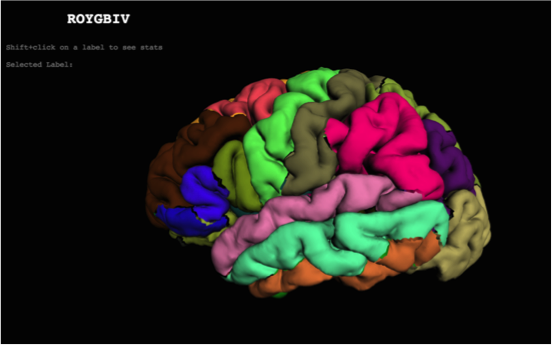
\includegraphics[width=.42\textwidth]{roygbiv.png}
  \caption{\label{centfig} Example visualization.}
\end{figure}

\section{Conclusions}\label{conclusions}

We have received very positive feedback on our efforts at the hackathon,
and have since received several requests and encouragement to build this
visualization out to accommodate other data besides shape information
and to enable the visual evaluation of thousands of brains. We hope to
continue this work with the help of others!

%%%%%%%%%%%%%%%%%%%%%%%%%%%%%%%%%%%%%%%%%%%%%%
%%                                          %%
%% Backmatter begins here                   %%
%%                                          %%
%%%%%%%%%%%%%%%%%%%%%%%%%%%%%%%%%%%%%%%%%%%%%%

\begin{backmatter}

\section*{Availability of Supporting Data}
More information about this project can be found at: \url{https://github.com/duecredit/duecredit}. Further data and files supporting this project are hosted in the \emph{GigaScience} repository REFXXX.

\section*{Competing interests}
None

\section*{Author's contributions}
KA and KA performed the project and wrote the report.

\section*{Acknowledgements}
The authors would like to thank the organizers and attendees of the 2015
OHBM Hackathon. This project is supported in part by a grant from the
NSF (award 1429999).

  
  
%%%%%%%%%%%%%%%%%%%%%%%%%%%%%%%%%%%%%%%%%%%%%%%%%%%%%%%%%%%%%
%%                  The Bibliography                       %%
%%                                                         %%
%%  Bmc_mathpys.bst  will be used to                       %%
%%  create a .BBL file for submission.                     %%
%%  After submission of the .TEX file,                     %%
%%  you will be prompted to submit your .BBL file.         %%
%%                                                         %%
%%                                                         %%
%%  Note that the displayed Bibliography will not          %%
%%  necessarily be rendered by Latex exactly as specified  %%
%%  in the online Instructions for Authors.                %%
%%                                                         %%
%%%%%%%%%%%%%%%%%%%%%%%%%%%%%%%%%%%%%%%%%%%%%%%%%%%%%%%%%%%%%

% if your bibliography is in bibtex format, use those commands:
\bibliographystyle{bmc-mathphys} % Style BST file
\bibliography{brainhack-report} % Bibliography file (usually '*.bib' )

\end{backmatter}
\end{document}
